% \documentclass[11pt,a4paper]{scrartcl}
\documentclass[class=minimal,border=0pt]{standalone}
\usepackage{tikz}
\usetikzlibrary{calc,math,arrows,positioning,shapes}
\usepackage{sfmath}
% \usepackage[fleqn]{amsmath}
% \usepackage{amssymb}
\usepackage{xspace}
% \usepackage[width=9.2cm, height=8.7cm,noheadfoot]{geometry}

\newcommand{\given}{\ensuremath{\,|\,}\xspace}
\newcommand{\pr}{\ensuremath{p}}

\newcommand{\data}{\ensuremath{D}\xspace}
\newcommand{\model}[1][]{\ensuremath{M_{#1}}\xspace}
\newcommand{\parameters}[1][]{\ensuremath{\Theta_{#1}}\xspace}
\newcommand{\parameter}[1][]{\ensuremath{\theta_{#1}}\xspace}
\newcommand{\diff}[1]{\ensuremath{\mathrm{d}#1}}

\newcommand{\distgamma}{\ensuremath{\textrm{Gamma}}\xspace}
\newcommand{\distexponential}{\ensuremath{\textrm{Exponential}}\xspace}
\newcommand{\dgamma}[2]{\ensuremath{\distgamma(\textrm{shape} = #1, \textrm{mean} = #2)}}
\newcommand{\dexponential}[1]{\ensuremath{\distexponential(\textrm{mean} = #1)}}

\newcommand{\ncomparisons}{\ensuremath{n\xspace}}
\newcommand{\nevents}[1][]{\ensuremath{k_{#1}\xspace}}
\newcommand{\nloci}[1][]{\ensuremath{m_{#1}\xspace}}

\newcommand{\observedallelecount}[1][]{\ensuremath{n_{#1}}\xspace}
\newcommand{\observedredallelecount}[1][]{\ensuremath{r_{#1}}\xspace}

\newcommand{\nodeallelecount}[2]{\ensuremath{n_{#1}^{#2}}}
\newcommand{\noderedallelecount}[2]{\ensuremath{r_{#1}^{#2}}}

\newcommand{\allelecount}[1][]{\ensuremath{\nodeallelecount{#1}{}}\xspace}
\newcommand{\redallelecount}[1][]{\ensuremath{\noderedallelecount{#1}{}}\xspace}

\newcommand{\leafallelecounts}[1][]{\ensuremath{\mathbf{n}_{#1}}\xspace}
\newcommand{\leafredallelecounts}[1][]{\ensuremath{\mathbf{r}_{#1}}\xspace}
\newcommand{\maxleafallelecounts}{\ensuremath{\textrm{max}(\mathbf{n})}\xspace}

\newcommand{\comparisondata}[1][]{\ensuremath{D_{#1}}\xspace}
\newcommand{\alldata}[1][]{\ensuremath{\mathbf{D}}\xspace}

\newcommand{\branchindex}{\ensuremath{x}\xspace}
\newcommand{\allelecountbottom}[1][\branchindex]{\nodeallelecount{#1}{B}}
\newcommand{\allelecounttop}[1][\branchindex]{\nodeallelecount{#1}{T}}
\newcommand{\redallelecountbottom}[1][\branchindex]{\noderedallelecount{#1}{B}}
\newcommand{\redallelecounttop}[1][\branchindex]{\noderedallelecount{#1}{T}}

\newcommand{\dppmsbayes}{\upshape\texttt{dpp-msbayes}\xspace}
\newcommand{\cpp}{\upshape\texttt{C++}\xspace}
\newcommand{\ecoevolity}{\upshape\texttt{ecoevolity}\xspace}
\newcommand{\timesizeratemixer}{\upshape\texttt{TimeSizeRateMixer}\xspace}
\newcommand{\timerootsizemixer}{\upshape\texttt{TimeRootSizeMixer}\xspace}
\newcommand{\simcoevolity}{\upshape\texttt{simcoevolity}\xspace}
\newcommand{\sumcoevolity}{\upshape\texttt{sumcoevolity}\xspace}
\newcommand{\pycoevolity}{\upshape\texttt{pycoevolity}\xspace}

\newcommand{\rgmurate}{\ensuremath{u}\xspace}
\newcommand{\grmurate}{\ensuremath{v}\xspace}
\newcommand{\murate}[1][]{\ensuremath{\mu_{#1}}\xspace}
\newcommand{\murates}[1][]{\ensuremath{\boldsymbol{\mu}_{#1}}\xspace}
\newcommand{\gfreq}[1][]{\ensuremath{\pi_{#1}}\xspace}
\newcommand{\gfreqs}[1][]{\ensuremath{\boldsymbol{\pi}_{#1}}\xspace}

\newcommand{\comparisondivtime}[1][]{\ensuremath{t_{#1}}\xspace}
\newcommand{\comparisondivtimes}[1][]{\ensuremath{\mathbf{t}_{#1}}\xspace}
\newcommand{\divtime}[1][]{\ensuremath{\tau_{#1}}\xspace}
\newcommand{\divtimes}[1][]{\ensuremath{\boldsymbol{\tau}_{#1}}\xspace}
\newcommand{\divtimemodel}[1][]{\ensuremath{T_{#1}}\xspace}
\newcommand{\divtimesets}{\ensuremath{\mathcal{T}}\xspace}
\newcommand{\genetree}[1][]{\ensuremath{g_{#1}}\xspace}
\newcommand{\sptree}[1][]{\ensuremath{S_{#1}}\xspace}
\newcommand{\sptrees}[1][]{\ensuremath{\mathbf{S}_{#1}}\xspace}

\newcommand{\descendantpopindex}[1]{\ensuremath{D{#1}}}
\newcommand{\rootpopindex}[1][]{\ensuremath{R{#1}}\xspace}
\newcommand{\epopsize}[1][]{\ensuremath{N_{e}^{#1}}\xspace}
\newcommand{\sepopsize}[1][]{\ensuremath{N}\xspace}
\newcommand{\comparisonpopsizes}[1][]{\ensuremath{\mathbb{N}_{e}{#1}}\xspace}
\newcommand{\collectionpopsizes}[1][]{\ensuremath{\mathbf{N_{e}}_{#1}}\xspace}
\newcommand{\rootrelativepopsize}{\ensuremath{R_{\epopsize[\rootpopindex]}}\xspace}

\newcommand{\dirp}{\ensuremath{\textrm{DP}}\xspace}
\newcommand{\concentration}{\ensuremath{\alpha}\xspace}
\newcommand{\basedistribution}{\ensuremath{H}\xspace}
\newcommand{\gshape}{\ensuremath{k}\xspace}
\newcommand{\gscale}{\ensuremath{\theta}\xspace}

\newcommand{\multiplier}{\ensuremath{m}\xspace}
\newcommand{\proposed}{\ensuremath{^{\prime}}\xspace}
\newcommand{\tuningparameter}{\ensuremath{\lambda}\xspace}
\newcommand{\uniformdeviate}{\ensuremath{u}\xspace}
\newcommand{\sizechange}{\ensuremath{\delta}\xspace}


\newcounter{cparametercounter}
\newcommand{\constantparameter}[1][]{%
    \stepcounter{cparametercounter}%
    \ensuremath{p^{#1}_{\arabic{cparametercounter}}}\xspace}

\begin{document}

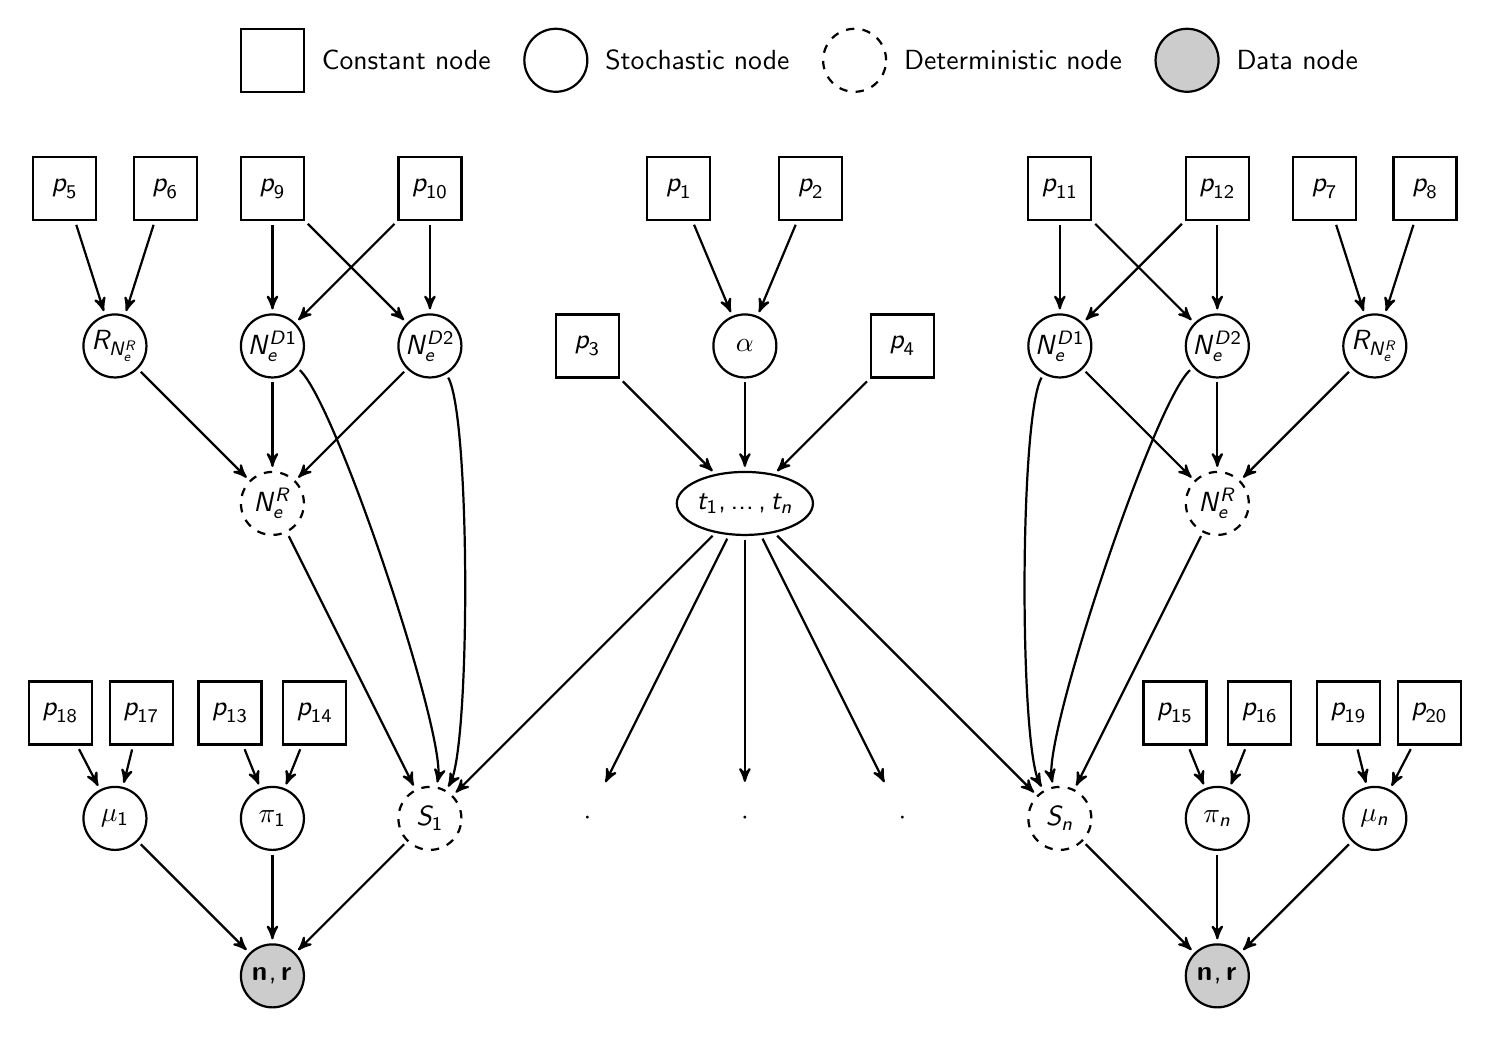
\begin{tikzpicture}[node distance = 2cm]
    \tikzstyle{dot} = [
            thick,
            text centered,
            minimum size = 8mm,
            inner sep = 0mm]
    \tikzstyle{dagnode} = [dot,
            draw,
            ]
    \tikzstyle{constant} = [dagnode,
            rectangle,
            fill=white]
    \tikzstyle{stochastic} = [dagnode,
            circle,
            fill=white]
    \tikzstyle{longstochastic} = [stochastic, ellipse]
    \tikzstyle{deterministic} = [dagnode,
            dashed,
            circle,
            fill=white]
    \tikzstyle{clamped} = [dagnode,
            circle,
            fill=black!20]
    \tikzstyle{dedge} = [->,
            >=stealth',
            thick,
            shorten <= 0.5mm,
            shorten >= 0.5mm,
            ]

    \node[stochastic] (conc) {\concentration};
    \node (abconcspace) [above of = conc] {};
    % \node[constant] (aconc) [left=3mm of abconcspace] {$a_{\concentration}$};
    % \node[constant] (bconc) [right=3mm of abconcspace] {$b_{\concentration}$};
    % \node[constant] (atime) [left of = conc] {$a_{\divtime}$};
    % \node[constant] (btime) [right of = conc] {$b_{\divtime}$};
    \node[constant] (aconc) [left=3mm of abconcspace] {\constantparameter};
    \node[constant] (bconc) [right=3mm of abconcspace] {\constantparameter};
    \node[constant] (atime) [left of = conc] {\constantparameter};
    \node[constant] (btime) [right of = conc] {\constantparameter};
    \node[longstochastic] (times) [below of = conc] {$\comparisondivtime[1], \ldots, \comparisondivtime[\ncomparisons]$};

    \node (sptree3above) [below of = times] {};
    \node (sptree2above) [left of = sptree3above] {};
    \node (sptree1above) [left of = sptree2above] {};
    \node (sptree4above) [right of = sptree3above] {};
    \node (sptreenabove) [right of = sptree4above] {};

    \node[dot] (sptree3) [below of = sptree3above] {$\cdot$};
    \node[dot] (sptree2) [below of = sptree2above] {$\cdot$};
    \node[deterministic] (sptree1) [below of = sptree1above] {\sptree[1]};
    \node[dot] (sptree4) [below of = sptree4above] {$\cdot$};
    \node[deterministic] (sptreen) [below of = sptreenabove] {\sptree[\ncomparisons]};


    \node (sptree1aboveabove) [above of = sptree1above] {};
    \node[deterministic] (rootpopsize1) [left of = sptree1aboveabove] {\epopsize[\rootpopindex]};
    \node[stochastic] (leaf1popsize1) [above of = rootpopsize1] {\epopsize[\descendantpopindex{1}]};
    \node[stochastic] (leaf2popsize1) [right of = leaf1popsize1] {\epopsize[\descendantpopindex{2}]};
    \node[stochastic] (relrootsize1) [left of = leaf1popsize1] {\rootrelativepopsize};
    \node (relrootsize1above) [above of = relrootsize1] {};
    % \node[constant] (arelsize1) [left=1mm of relrootsize1above] {$a^1_{\rootrelativepopsize}$};
    % \node[constant] (brelsize1) [right=1mm of relrootsize1above] {$b^1_{\rootrelativepopsize}$};
    \node[constant] (arelsize1) [left=1mm of relrootsize1above] {\constantparameter};
    \node[constant] (brelsize1) [right=1mm of relrootsize1above] {\constantparameter};

    \node (sptreenaboveabove) [above of = sptreenabove] {};
    \node[deterministic] (rootpopsizen) [right of = sptreenaboveabove] {\epopsize[\rootpopindex]};
    \node[stochastic] (leaf1popsizen) [above of = rootpopsizen] {\epopsize[\descendantpopindex{2}]};
    \node[stochastic] (leaf2popsizen) [left of = leaf1popsizen] {\epopsize[\descendantpopindex{1}]};
    \node[stochastic] (relrootsizen) [right of = leaf1popsizen] {\rootrelativepopsize};
    \node (relrootsizenabove) [above of = relrootsizen] {};
    % \node[constant] (arelsizen) [left=1mm of relrootsizenabove] {$a^{\ncomparisons}_{\rootrelativepopsize}$};
    % \node[constant] (brelsizen) [right=1mm of relrootsizenabove] {$b^{\ncomparisons}_{\rootrelativepopsize}$};
    \node[constant] (arelsizen) [left=1mm of relrootsizenabove] {\constantparameter};
    \node[constant] (brelsizen) [right=1mm of relrootsizenabove] {\constantparameter};

    % \node[constant] (apopsize1) [above of = leaf1popsize1] {$a^1_{\epopsize[\descendantpopindex{}]}$};
    % \node[constant] (bpopsize1) [above of = leaf2popsize1] {$b^1_{\epopsize[\descendantpopindex{}]}$};
    \node[constant] (apopsize1) [above of = leaf1popsize1] {\constantparameter};
    \node[constant] (bpopsize1) [above of = leaf2popsize1] {\constantparameter};

    % \node[constant] (bpopsizen) [above of = leaf1popsizen] {$b^{\ncomparisons}_{\epopsize[\descendantpopindex{}]}$};
    % \node[constant] (apopsizen) [above of = leaf2popsizen] {$a^{\ncomparisons}_{\epopsize[\descendantpopindex{}]}$};
    \node[constant] (apopsizen) [above of = leaf2popsizen] {\constantparameter};
    \node[constant] (bpopsizen) [above of = leaf1popsizen] {\constantparameter};

    \node (gfreq1above) [left of = sptree1above] {};
    \node (murate1above) [left of = gfreq1above] {};

    \node (gfreqnabove) [right of = sptreenabove] {};
    \node (muratenabove) [right of = gfreqnabove] {};

    \node[stochastic] (gfreq1) [below of = gfreq1above] {\gfreq[1]};
    \node[stochastic] (murate1) [below of = murate1above] {\murate[1]};

    \node[stochastic] (gfreqn) [below of = gfreqnabove] {\gfreq[\ncomparisons]};
    \node[stochastic] (muraten) [below of = muratenabove] {\murate[\ncomparisons]};

    \node[clamped] (pattern1) [below of = gfreq1] {$\leafallelecounts, \leafredallelecounts$};

    \node[clamped] (patternn) [below of = gfreqn] {$\leafallelecounts, \leafredallelecounts$};

    \node (gfreq1above) [above=8mm of gfreq1] {};
    % \node[constant] (agfreq1) [left=0mm of gfreq1above] {$a^1_{\gfreq}$};
    % \node[constant] (bgfreq1) [right=0mm of gfreq1above] {$b^1_{\gfreq}$};
    \node[constant] (agfreq1) [left=0mm of gfreq1above] {\constantparameter};
    \node[constant] (bgfreq1) [right=0mm of gfreq1above] {\constantparameter};

    \node (gfreqnabove) [above=8mm of gfreqn] {};
    % \node[constant] (agfreqn) [left=0mm of gfreqnabove] {$a^{\ncomparisons}_{\gfreq}$};
    % \node[constant] (bgfreqn) [right=0mm of gfreqnabove] {$b^{\ncomparisons}_{\gfreq}$};
    \node[constant] (agfreqn) [left=0mm of gfreqnabove] {\constantparameter};
    \node[constant] (bgfreqn) [right=0mm of gfreqnabove] {\constantparameter};

    % \node[constant] (bmurate1) [left=3mm of agfreq1] {$b^1_{\murate}$};
    % \node[constant] (amurate1) [left=2mm of bmurate1] {$a^1_{\murate}$};
    \node[constant] (bmurate1) [left=3mm of agfreq1] {\constantparameter};
    \node[constant] (amurate1) [left=2mm of bmurate1] {\constantparameter};

    % \node[constant] (amuraten) [right=3mm of bgfreqn] {$a^{\ncomparisons}_{\murate}$};
    % \node[constant] (bmuraten) [right=2mm of amuraten] {$b^{\ncomparisons}_{\murate}$};
    \node[constant] (amuraten) [right=3mm of bgfreqn] {\constantparameter};
    \node[constant] (bmuraten) [right=2mm of amuraten] {\constantparameter};


    % Key
    \node[constant] (keyconstant) [above=0.8cm of apopsize1] {};
    \node[dot] (keyconstanttext) [right=2mm of keyconstant] {\sffamily Constant node};
    \node[stochastic] (keystochastic) [right=4mm of keyconstanttext] {}; 
    \node[dot] (keystochastictext) [right=2mm of keystochastic] {\sffamily Stochastic node};
    \node[deterministic] (keydeterministic) [right=4mm of keystochastictext] {};
    \node[dot] (keydeterministictext) [right=2mm of keydeterministic] {\sffamily Deterministic node};
    \node[clamped] (keyclamped) [right=4mm of keydeterministictext] {};
    \node[dot] (keyclampedtext) [right=2mm of keyclamped] {\sffamily Data node};


    \draw[dedge] (aconc) -- (conc);
    \draw[dedge] (bconc) -- (conc);
    \draw[dedge] (conc) -- (times);
    \draw[dedge] (atime) -- (times);
    \draw[dedge] (btime) -- (times);

    \draw[dedge] (times) -- (sptree1);
    \draw[dedge] (times) -- (sptree2);
    \draw[dedge] (times) -- (sptree3);
    \draw[dedge] (times) -- (sptree4);
    \draw[dedge] (times) -- (sptreen);

    % \draw[dedge] (sptree1) to [bend left] node[right] {$\int_{\genetree}$} (pattern1);
    \draw[dedge] (sptree1) -- (pattern1);
    \draw[dedge] (gfreq1) -- (pattern1);
    \draw[dedge] (murate1) -- (pattern1);

    \draw[dedge] (arelsize1) -- (relrootsize1);
    \draw[dedge] (brelsize1) -- (relrootsize1);

    \draw[dedge] (apopsize1) -- (leaf1popsize1);
    \draw[dedge] (apopsize1) -- (leaf2popsize1);
    \draw[dedge] (bpopsize1) -- (leaf1popsize1);
    \draw[dedge] (bpopsize1) -- (leaf2popsize1);

    \draw[dedge] (relrootsize1) -- (rootpopsize1);
    \draw[dedge] (leaf1popsize1) -- (rootpopsize1);
    \draw[dedge] (leaf2popsize1) -- (rootpopsize1);

    \draw[dedge] (rootpopsize1) -- (sptree1);
    \draw[dedge] (leaf1popsize1) to [bend left, looseness=0.3] (sptree1);
    \draw[dedge] (leaf2popsize1) to [bend left, looseness=0.3] (sptree1);

    \draw[dedge] (amurate1) -- (murate1);
    \draw[dedge] (bmurate1) -- (murate1);

    \draw[dedge] (agfreq1) -- (gfreq1);
    \draw[dedge] (bgfreq1) -- (gfreq1);


    % \draw[dedge] (sptreen) to [bend right] node[left] {$\int_{\genetree}$} (patternn);
    \draw[dedge] (sptreen) -- (patternn);
    \draw[dedge] (gfreqn) -- (patternn);
    \draw[dedge] (muraten) -- (patternn);

    \draw[dedge] (arelsizen) -- (relrootsizen);
    \draw[dedge] (brelsizen) -- (relrootsizen);

    \draw[dedge] (apopsizen) -- (leaf1popsizen);
    \draw[dedge] (apopsizen) -- (leaf2popsizen);
    \draw[dedge] (bpopsizen) -- (leaf1popsizen);
    \draw[dedge] (bpopsizen) -- (leaf2popsizen);

    \draw[dedge] (relrootsizen) -- (rootpopsizen);
    \draw[dedge] (leaf1popsizen) -- (rootpopsizen);
    \draw[dedge] (leaf2popsizen) -- (rootpopsizen);

    \draw[dedge] (rootpopsizen) -- (sptreen);
    \draw[dedge] (leaf1popsizen) to [bend right, looseness=0.3] (sptreen);
    \draw[dedge] (leaf2popsizen) to [bend right, looseness=0.3] (sptreen);

    \draw[dedge] (amuraten) -- (muraten);
    \draw[dedge] (bmuraten) -- (muraten);

    \draw[dedge] (agfreqn) -- (gfreqn);
    \draw[dedge] (bgfreqn) -- (gfreqn);

\end{tikzpicture}
\end{document}
